\section{习题参考答案}
\subsection*{计算题}
\begin{enumerate}
    \item 如图所示~\ref{Fig:96},长直导线中通有电流$I=5.0A$,另一矩形线圈共1000匝,宽$a=10\mathrm{cm}$,长$L=20\mathrm{cm}$,以$v=2\mathrm{m/s}$的速度向右平动,求当$d=10\mathrm{cm}$时线圈中的感应电动势。
    \insertfig{0.3}{fig96}{Fig:96}
    \begin{solution}
        如图:
        \begin{figure}[H]
            \centering
            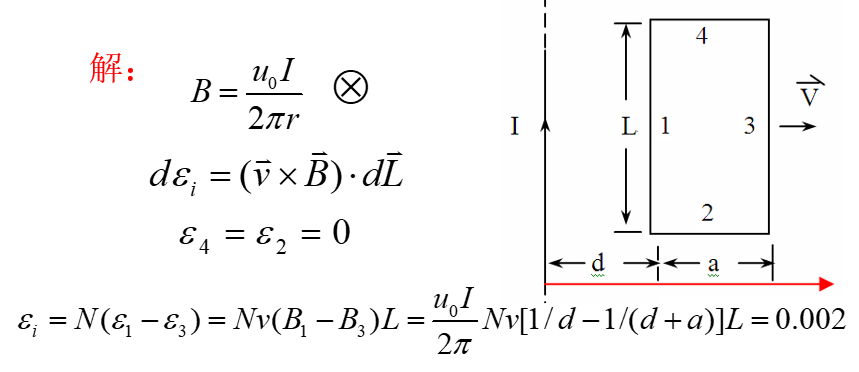
\includegraphics[width=0.55\textheight]{ans69}
        \end{figure}
    \end{solution}
    \item 如图~\ref{Fig:79}~半径分别为~$R$~和~$r$~的金属圆环共轴放置,且$R>>r$ ,在大圆环中有恒定电流,而小圆环则以恒定速度沿轴线方向运动,求当小圆环与大圆环相距$X$时小圆环中的电动势大小。
    \insertfig{0.3}{fig97}{Fig:97}
    \begin{solution}
        如图:
        \begin{figure}[H]
            \centering
            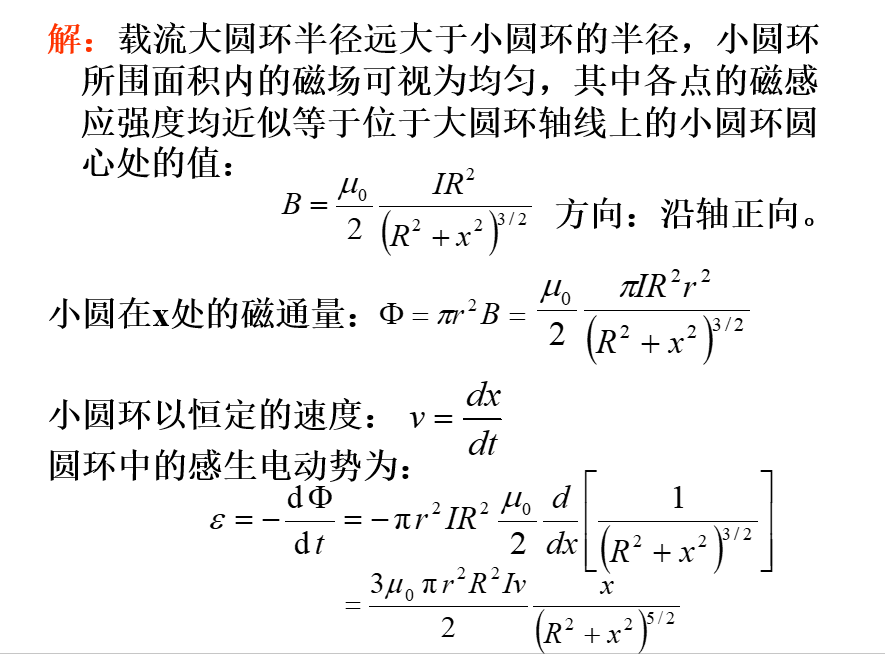
\includegraphics[width=0.55\textheight]{ans70}
        \end{figure}
    \end{solution}
    \item 如图~\ref{Fig:98}~一半径为$a$的非常小的金属圆环,$t=0$时,它与一半径为$b$~($b>>a$)的金属圆环共面且同心,今在大环中通以恒定电流$I$,而小环以角速度~$\omega$~绕其一直径匀角速转动,小环电阻为$R$. 求:
    \begin{enumerate}[label=(\arabic*)]
        \item  $t$时刻穿过小环的磁通量.
        \item 小环中的感应电流.
    \end{enumerate}
    \insertfig{0.3}{fig98}{Fig:98}
    \begin{solution}
        如图:
        \begin{figure}[H]
            \centering
            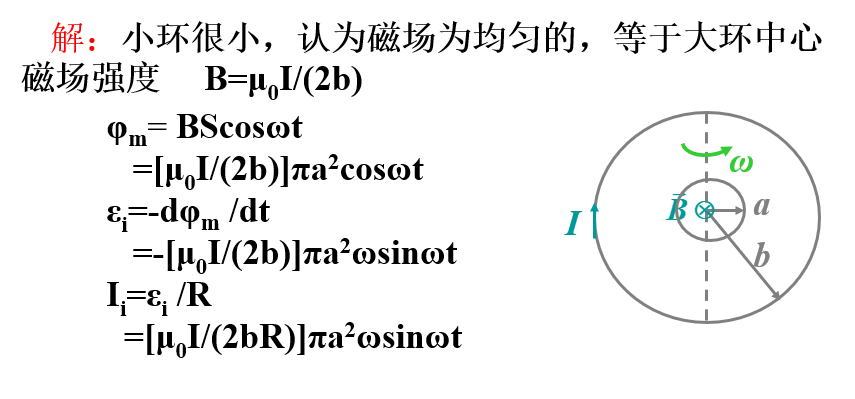
\includegraphics[width=0.55\textheight]{ans71}
        \end{figure}
    \end{solution}
    \item 如图所示~\ref{Fig:99},一通有交变电流$I=I_0\mathrm{sin}\omega t$的长直导线旁有一共面的矩形线圈,试求:
    \begin{enumerate}[label=(\arabic*)]
        \item 穿过线圈回路的磁通量;
        \item 回路中感应电动势大小。
    \end{enumerate}
    \insertfig{0.3}{fig99}{Fig:99}
    \begin{solution}
        如图:
        \begin{figure}[H]
            \centering
            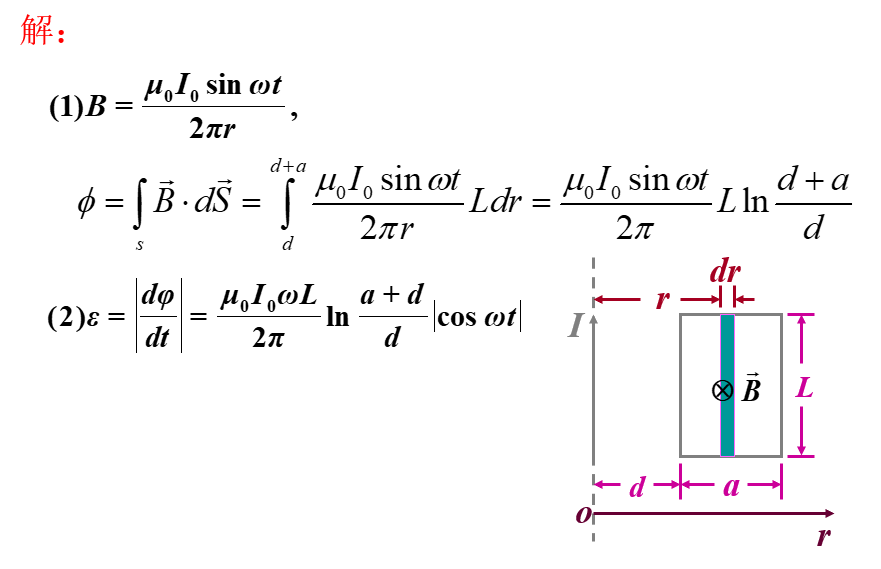
\includegraphics[width=0.55\textheight]{ans72}
        \end{figure}
    \end{solution}
\end{enumerate}